% !TeX spellcheck = en_US
\documentclass[]{article}

\usepackage[utf8]{inputenc}

\usepackage{natbib}
\usepackage{graphicx}

\usepackage[english]{babel}
\usepackage{amsmath}
\usepackage{amsfonts}
\usepackage{amssymb}

\usepackage[T1]{fontenc}
\usepackage{listingsutf8}
\lstset{literate={č}{{\v c}}1 {š}{{\v s}}1 {ž}{{\v z}}1}
\lstset{basicstyle=\ttfamily, language=matlab}


\title{Homework 1}
\author{Lovro Habjan}

\begin{document}

\maketitle


\section{Introduction}

For homework 1 we implemented iterative methods for tridiagonal matrices. We
wrote functions for \textit{Jacobi}, \textit{Gaus-Seidel} and \textit{SOR}
iterations.

\section{Methods}

Our goal is to solve the system $Ax = \mathbf{b}$ where $A \in \mathbb{R}^{n
\times n}$ is a tridiagonal matrix. For example
\begin{equation*}
	A = \begin{bmatrix}
		1 & 2 & 2 & 0 \\
		3 & 4 & 5 & 0 \\
		0 & 6 & 7 & 8 \\
		0 & 0 & 9 & 10
	\end{bmatrix}
\end{equation*}
which we can represent with matrix
\begin{equation*}
	M = \begin{bmatrix}
		0 & 1 & 2 \\
		3 & 4 & 5 \\
		6 & 7 & 8 \\
		9 & 10 & 0
	\end{bmatrix}
\end{equation*}

Because of this our iterative methods are easier to compute. If we observe the
equation for the Jacobian iteration
\begin{equation*}
	x_i^{(k+1)} = \frac{1}{a_{ii}} \left( b_i - \sum_{j = 1}^{i-1} a_{ij}
		x_j^{(k)} - \sum_{j = i + 1}^{n} a_{ij} x_j^{(k)} \right)
\end{equation*}
we observe that all elements $a_{i1}, a_{i2}, ..., a_{i i-2}, a_{i i + 2},
a_{i i + 3}, ..., a_{i n}$ equal 0 because $A$ is tridiagonal. This gives us
simpler equations for all three methods. Jacobian iteration looks like
\begin{equation*}
	x_i^{(k+1)} = \frac{1}{a_{ii}} \left( b_i - a_{i i-1} x_{i-1}^{(k)} -
		a_{i i+1} x_{i+1}^{(k)} \right),
\end{equation*}
Gauss-Seidel iteration as
\begin{equation*}
	x_i^{(k+1)} = \frac{1}{a_{ii}} \left( b_i - a_{i i-1} x_{i-1}^{(k+1)} -
		a_{i i+1} x_{i+1}^{(k)} \right)
\end{equation*}
and SOR iteration as
\begin{equation*}
	x_i^{(k+1)} = \frac{\omega}{a_{ii}} \left( b_i - a_{i i-1} x_{i-1}^{(k+1)} -
		a_{i i+1} x_{i+1}^{(k)} \right) + (1 - \omega) x_i^{(k)}
\end{equation*}


We use the maximum norm to stop the iteration when we achieve satisfactory
accuracy:
\begin{equation*}
	\Vert Ax^{(k)} - \mathbf{b} \Vert_{\infty} < acc
\end{equation*}


\section{Results}

All three methods are implemented in \textit{iter3.m} file. We count the number
of iterations for each method.

We tested our implementation with the following system:
\begin{equation*}
		A = \begin{bmatrix}
	2 & -1 & 0 & 0 \\
	-1 & 2 & -1 & 0 \\
	0 & -1 & 2 & -1 \\
	0 & 0 & -1 & 2
	\end{bmatrix}
\end{equation*}
which takes the form:
\begin{equation*}
	M = \begin{bmatrix}
		0 & 2 & -1 \\
		-1 & 2 & -1 \\
		-1 & 2 & -1 \\
		-1 & 2 & 0
	\end{bmatrix}
\end{equation*}
We define the solution and the initial guess as:
\begin{align*}
	\mathbf{b} = \begin{bmatrix}
		1 \\ 0 \\ 0 \\ 1
	\end{bmatrix}
	&
	x_0 = \begin{bmatrix}
		0 \\ 0 \\ 0 \\ 0
	\end{bmatrix}
\end{align*}

If we set $\omega = 1$, we get the same number of iterations as for the
Gauss-Seidel method. Example for $\omega = 1.3$:

\begin{lstlisting}
>> [x, j, g, s] = iter3(M, b, x0, 1e-6, 1.3)
x = [1.0000; 1.0000; 1.0000; 1.0000]
j = 62
g = 33
s = 19
\end{lstlisting}

With higher precision:

\begin{lstlisting}
>> [x, j, g, s] = iter3(M, b, x0, 1e-13, 2)
x = [1; 1; 1; 1]
j = 138
g = 71
s = 1
\end{lstlisting}

Different values of $\omega$ are shown in figure \ref{fig:1-omega}. The optimal
value occurs at $\omega = 2$ followed by a big spike.

Figure \ref{fig:1-acc} shows the number of iterations in respect to desired
accuracy for all three methods. For SOR method we used $\omega = 1.5$. We see
that Jacobian method performs the worst, with exponential growth of iterations
for all methods when the accuracy approaches 0.

The test code is located in \textit{test.m} file.

\begin{figure}
	\centering
	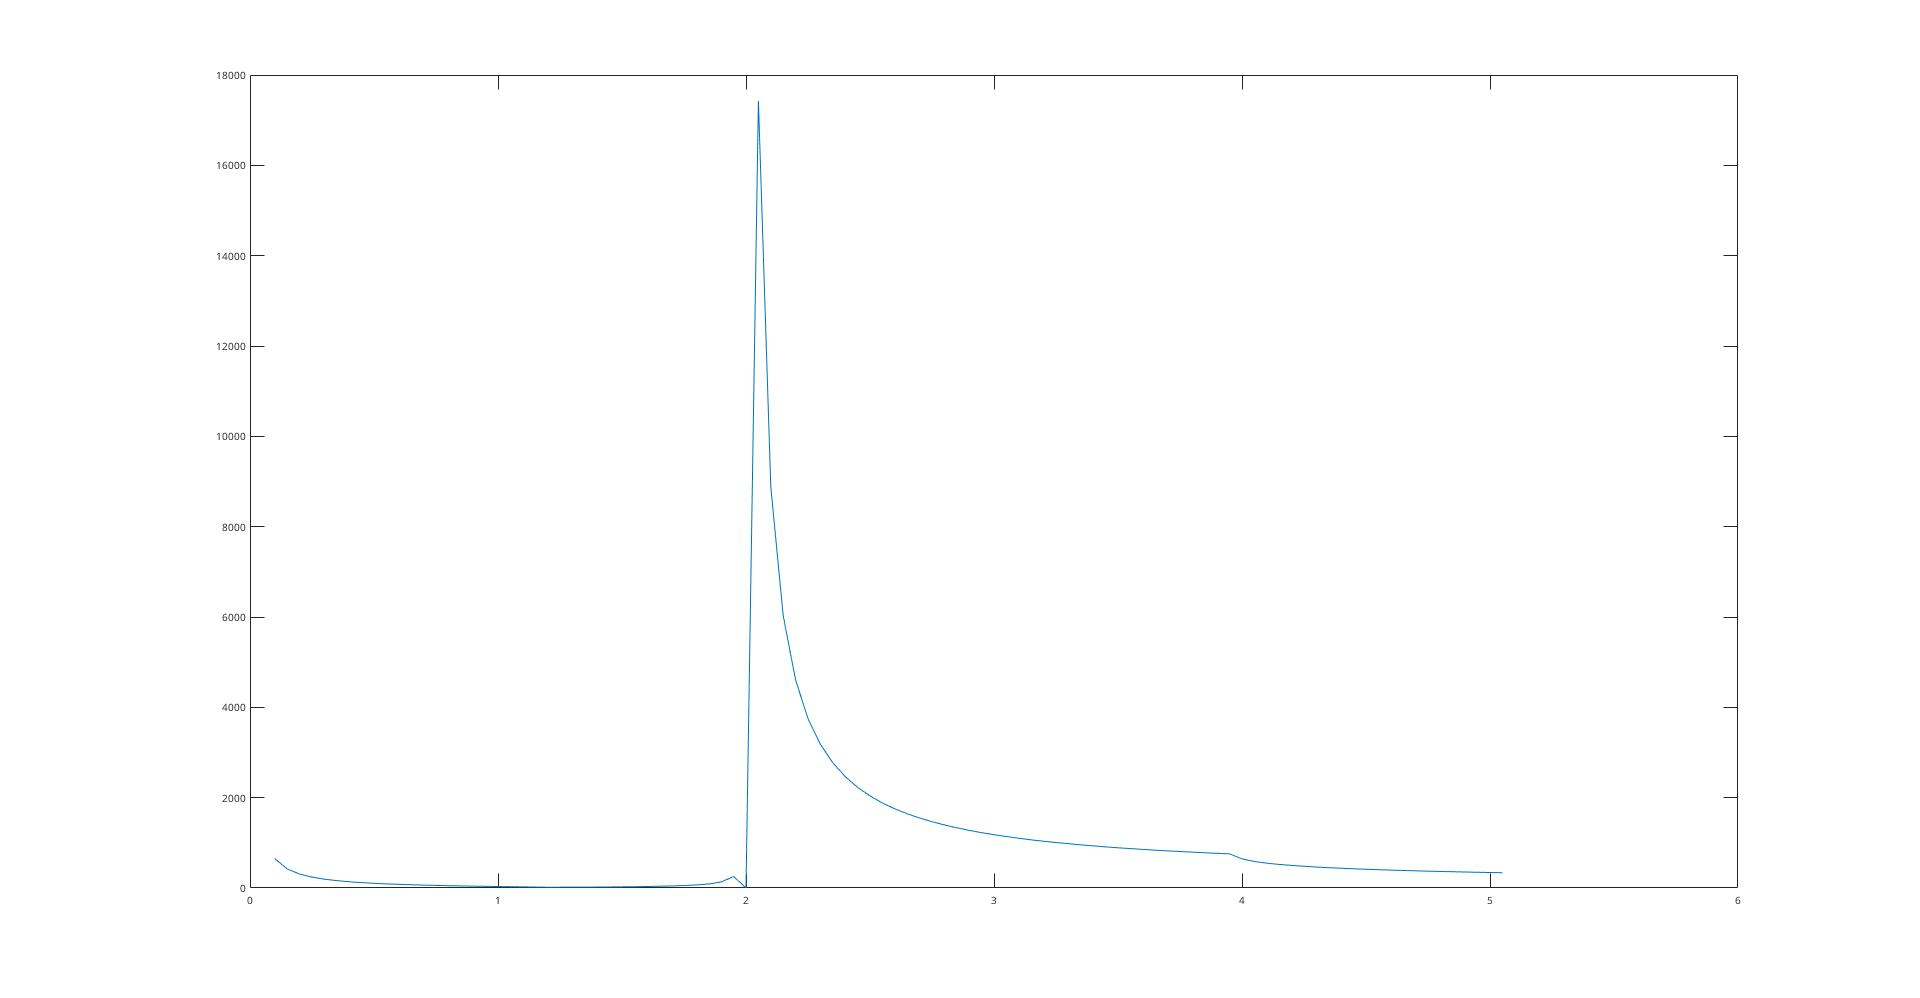
\includegraphics[width=\linewidth]{pics/test1omega.jpg}
	\caption{Number of iterations for SOR method with different values of $\omega$}
	\label{fig:1-omega}
\end{figure}

\begin{figure}
	\centering
	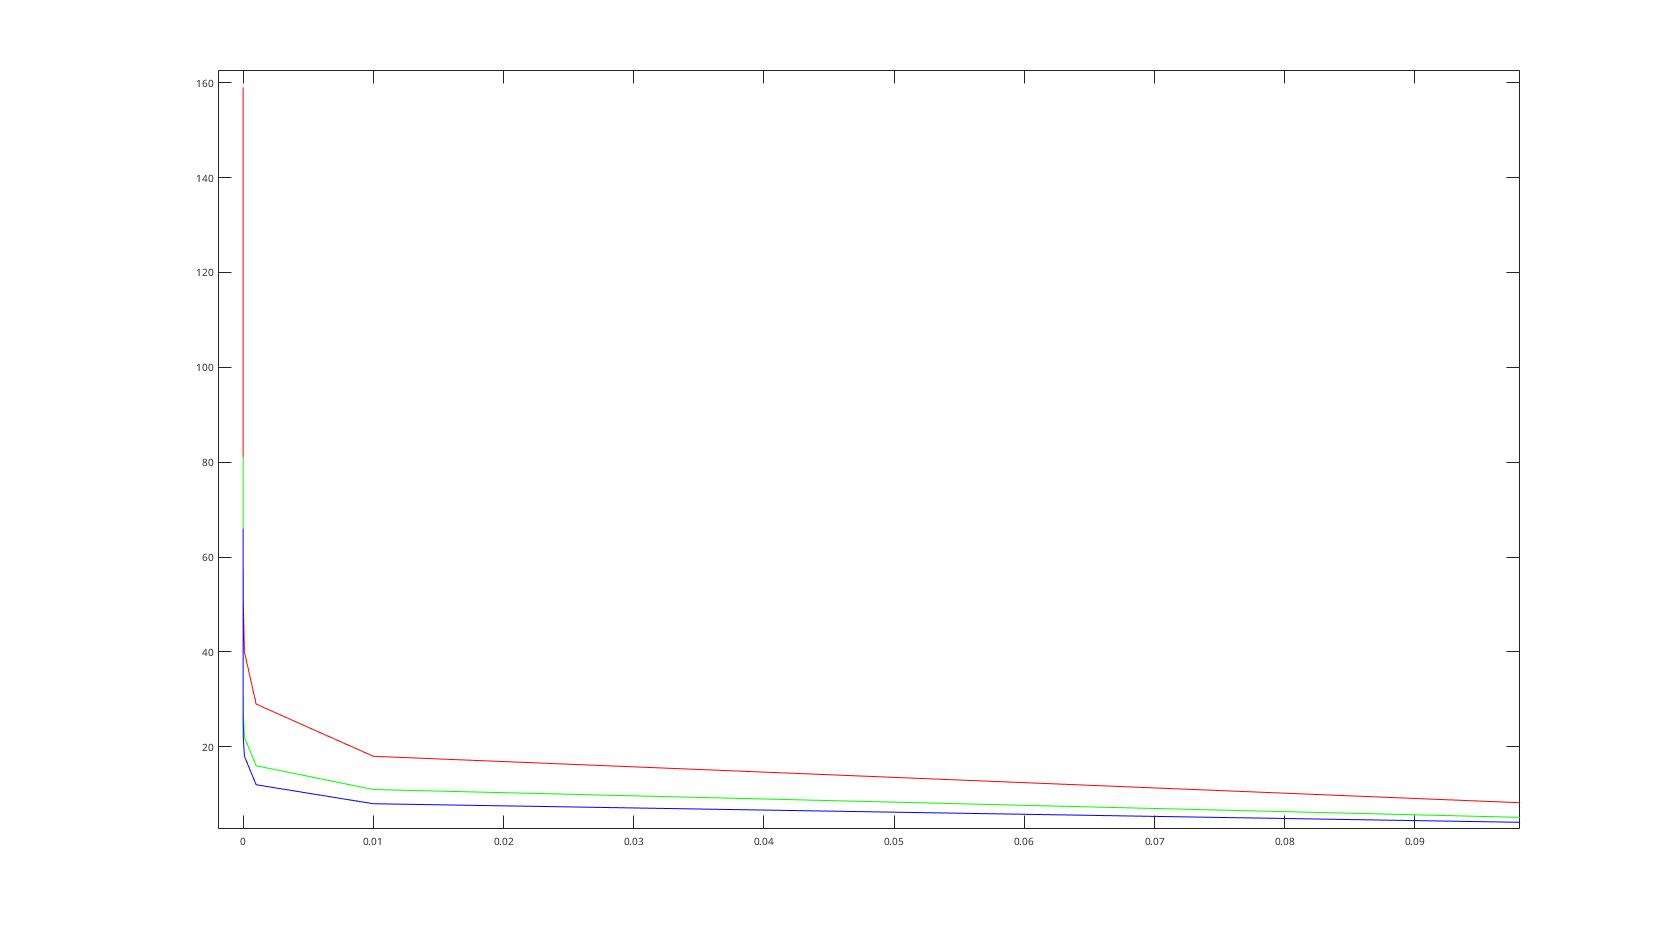
\includegraphics[width=\linewidth]{pics/test1-acc.jpg}
	\caption{Number of iterations for Jacobian, Gauss-Seidel and SOR method with
		different values of accuracy}
	\label{fig:1-acc}
\end{figure}


\end{document}
